% !TEX encoding = UTF-8 Unicode
% !TEX program = pdflatex
% !TEX spellcheck = en_US


% In order to correctly compile this document,
% execute the following commands:
% 1. pdflatex
% 2. pdflatex
% 3. pdflatex



\documentclass[amsthm,ebook]{saparticle}

% IF YOU USE PDFLATEX
\usepackage[utf8x]{inputenc}
% if you write in english and in greek
\usepackage{ucs}
\usepackage[greek,english]{babel}
\languageattribute{greek}{polutoniko}

% IF YOU USE XELATEX
%\usepackage{polyglossia}
% if you write in italian
%\setmainlanguage{italian}
% If you want put some ancient greek:
%\setotherlanguage[variant=polytonic]{greek}
%\newfontfamily{\greekfont}[Ligatures=TeX]{Palatino Linotype}

% dummy text (remove in a normal thesis)
% remove if not necessary
\usepackage{siunitx}
%Natbib for bibliography management
\usepackage[authoryear]{natbib}
% custom commands
\newcommand{\bs}{\textbackslash}

%%%%%%%%
%TITLE:%
%%%%%%%%
\title{The Power of Images at Aphrodisias: 
How Digital Resources Can Transform our assessment of Palaeography}
\author[war]{Abigail S. Graham\corref{first}}
\address[war]{The University of Warwick}
\cortext[first]{Corresponding author. Email: Abigail.graham@warwick.ac.uk}
\date{2015-11-16}
\begin{document}
 \maketitle
\begin{abstract}
This paper will consider how the publication of a large digital corpus The Inscriptions of Aphrodisias \citet{ReynoldsRouecheBodard2007} has shaped the assessment of inscriptions, particularly regarding palaeography and the dating
of inscriptions. A case study of dedicatory inscriptions from the Temple of Aphrodite at Aphrodisias will explore how
our approach to palaeography and dating has evolved with digital resources, identifying areas where challenges remain
and considering how improvements could be made in both our approach to and in publication of epigraphic materials. 

\end{abstract}
\keywords{Dating, Palaeography, Ordinatio, Letter forms, Aphrodisias, Context, Recarving.}


\section{Introduction}
\subsection{Caveat Lector: Defining Palaeography and traditional approaches}

\noindent  As the co-ordinator and lecturer on three graduate level courses of Roman Epigraphy, I am invariably asked the same
question: how do you use letterforms to date inscriptions? My answer is always the same: ``very carefully''. Studying
palaeography within the discipline of ancient epigraphy can be a journey into thorny hedge where one can easily ``fall
into that category of human endeavor known as stylistic attribution and inevitably involve subjectivity''.\footnote{\citet[3-4]{tracy1995}} Stephen Tracy advises that palaeographic surveys should be carried out with caution: ``Caveat Lector
must needs be our motto''. The study of palaeography is problematic, as demonstrated by W. Eck and C. Roueché during the conference, on a number of levels, both in the way it is
defined and the ways in which it is employed. Many scholars dismiss lettering as a means of dating and they make an
important point: dating by a single criterion, especially a stylistic one, is somewhat precarious. When studied in
isolation, letterforms present stylistic variations that may be characteristic of a specific individual, workshop or an
urban area. While observations about carving techniques can be helpful in specific case studies, they are more
problematic when applied generally on a broader scale (e.g. to larger geographical areas or time trame) where
archaisms, local styles, and variations can create distortions.\footnote{\citet{susini1973}; \citet{petrucci1993}; \citet[163-181]{Manzella1995}; \citet[433]{cooley2012}; \citet[122-125]{bruun2015}.} Similar caution would be applied in dating a
sculpture on the basis of a hair fragment. Analysis of statues considers a number of factors, material, hairstyle,
drapery and/or context. Inscriptions are doubly difficult, as they fall into categories of both text and an object.
While there is potentially more information, there is also a greater chance that it will be contradictory. Thus the use
of lettering, an ``imprecise science'', is better used in combination with a number of different factors.\footnote{\citet[26-9]{harris1989}; \citet[3-5]{bodel2001}; \citet[393-418]{Manzella2007} and \citet[432-435]{cooley2012}.} Despite the
aforementioned limitations, a number of informative palaeographic studies have been produced. The success of these is
based on detailed commentaries on a specific corpus of material, a transparent methodology and the incorporation of
numerous high quality images.\footnote{ For example: \citet{Gordon1957} offers more than 50 plates and figures, \citet{Manzella1987} provides 218 illustrations, \citet{tracy1990,tracy1995,tracy2003} uses over 60 plates and figures in each volume.}





A second issue in the study of palaeography involves the access and publication of epigraphic materials. Access to
large corpora of inscriptions has traditionally been limited to a small audience of scholars and site visitors. Apart
from a few museum collections, which happen to have inscriptions arranged in roughly chronological order,\footnote{
Perhaps the finest example of a museum in which one can gain and understanding of palaeography (and inscriptions as
whole) is the Museo Epigrafico Nazionale, Roma. } there are few places where one can visually experience the
development of carving styles over time. For the lucky few who attain access (and permission) to study a large corpus
of inscriptions, publishing these texts with supporting images can be challenging and expensive. Studies of
palaeography in ancient inscriptions have often been, by necessity, selective with images making it difficult for both
the author and readers to develop a detailed understanding of carving trends and practices. In this traditional format,
inscriptions were also separated from their archaeological context and the accompanying artwork while the reader,
viewing only the lettering, was often removed from the visual elements of the inscription (e.g. the type of stone, use
of spacing and decoration, letter size). This is a suboptimal way of assessing epigraphic evidence. 
\vspace{5pt}
The advent of online corpora have increased both the access and the development of discussions regarding epigraphic
monumentality, including new methodologies, approaches as well as attempts to redefine genre classifications and
terminology.\footnote{\citet[22-39]{woolf1996}, \citet{eck2010}, \citet[1-10]{panciera2012}, \citet[1-17]{graham2013}. For a recent collection and analysis of epigraphic databases, see \citet[78-85]{Elliot2015}.} A
number of recent studies have used changes in the appearance of inscriptions over time, such as the use of different
media, decorative and paratextual elements\footnote{On marks in the text see \citet[26]{susini1973} and \citet[143-155]{cooley2014}.} (e.g. ivy leaves as interpuncts (hederae distinguentes),\footnote{\citet[293-303]{hommel1970}}
abbreviations\footnote{\citet[111]{Gordon1957}} and spacing between words\footnote{On using
space to reconstruct inscriptions see \citet[195-226]{alfoldy1995}, \citet[151-176]{grasby2002}.} alongside lettering, as dating
criteria.\footnote{ For an extensive list of dating conventions cf. \citet[Chapter 20]{Manzella1987}. }
Panciera’s recent article, in particular, advocates the significance of the public context and visibility of
inscriptions.\footnote{ ``I would propose to regard as an ‘inscription’ any particular type of written human
communication of the sort that we would today call unidirectional…not being addressed to a person or to a group but to
a collectivity, and for this reason is made with the location, writing technique, graphic form and impagination, mode
and register of expression chosen because they are most suitable to the attainment of its intended goal.'' \citep[8]{panciera2012}.} In this vein, it is worth considering how the physical characteristics of an inscription belong within a
broader assessment of a culture of writing. Is palaeography the study of letterforms alone? Was a focus on letterforms
a deliberate choice or a product of the traditional constraints in accessibility and publication of epigraphic
materials? The following case study from Aphrodisias will explore these questions further. 




\subsection{Outline}


\noindent The focus of this paper is a series of rather unimpressive column dedications from the temple of Aphrodite at
Aphrodisias. While the information recorded in the texts is unremarkable, the journey of these inscriptions from a paper epigraphic corpus to their recent publication as a digital corpus reveals an epic transformation in the
format and approach to these materials. This study will begin with brief overview of previous published editions
(e.g. \citet{calder1962}) followed by an assessment of the information available on the current Inscriptions of
Aphrodisias (2007) website. Through careful assessment of text (including formula, vocabulary and spelling) and its
presentation (the arrangement of the text, use of decoration and spaces, as well as lettering) in the images provided,
this survey will demonstrate how the availability of published images and inclusion of dating criteria have increased
the amount of information available whilst also adding clarity to the process of dating an inscription. By examining
how we define and use palaeography to evaluate inscriptions on the Inscriptions of Aphrodisias website \citep{ReynoldsRouecheBodard2007}, we
can observe how the discipline has evolved and what changes may be possible in approaches and the publication of
epigraphic material. 

%%%%%%%%%
%IN THE DOC THERE IS A "BOX" WITH this text
%Key Questions:
%
%What elements of the text are available to us in different media?
%How do we record the dating process and criteria? 
%How do we represent (and attempt to reconcile) contradictory information?
%%%%%%%%%%%

\vspace{5pt}
\section{Publishing inscriptions: A Case Study of Column Dedications from The Temple Of Aphrodite at Aphrodisias}

\subsection{A brief introduction to the inscriptions IAph 1.4-1.6.}


\noindent Three inscriptions, each of which record the dedication of a column at the Temple of Aphrodite, will be the subject of
this survey. The first two texts were noted as early as the 18th century and copied in a notebook by the British
Architect Deering in the early 19th century. A third version of the text, was uncovered during excavations at the
temple site by the French Engineer Gaudin in the early 20th century.\footnote{ A comprehensive history of the history
and bibliography, as well as a description of the resources can be found on the IAph website:
\url{http://insaph.kcl.ac.uk/iaph2007/iAph010006.html}. } The inscriptions are recorded on tabella ansata (0.745 x 0.465m) as
part of fluted marble columns of the peristasis, some of these have been reconstructed in modern restorations on the
site. 




These texts can be dated through a number of different criteria. Contextual association with construction of the
temple, dates between the end of the 1st century BC and the early 1st century AD, though the land was clearly in use
well before this time. \footnote{\citet[41-42]{smith1996} and \citet[37]{reynolds1990}. References to Sulla’s dedications are in
Appian BC 1.97. Caesar and Augustus’ acknowledgements of the sacred space are evident in IAph 8.27, 8.31 and 1.1. }
This is corroborated by coins depicting the temple, which date from 2 BC- 14 AD.\footnote{ Coin type 41 depicts
Augustus (OBV) and the temple of Aphrodite (REV) in MacDonald 1992, Plate V R131. } Prosopography is also informative:
Gaius Julius Zoilos (freed by Caesar or Octavian), who dedicated the theatre at Aphrodisias ca. 28 BC, also dedicated
the naos of the temple (IAph 1.2), perhaps posthumously. \footnote{ The titles on the architrave inscription, soter and
euergetes, are absent from Zoilos’ other inscriptions and may imply a posthumous dedication, perhaps by the boule and
demos \citep[38]{reynolds1990}.} The benefactor of the columns in this case study, Eumachos Diogenes, also comes from an
established family that flourished well into the 2nd century AD.\footnote{The success of Eumachus Diogenes’ family,
which included the first known Aphrodisian to hold a procuratorship in the 2nd century AD, reveals an enduring
significance for his family monuments in the city \citep[327-334]{reynolds1999}.} Finally, the formula of the text the
inscription and the vocabulary, particularly the term philokaisar, suggest a late Republican or Augustan
date.\footnote{ The formula of the dedication, which lists the benefactor first is evident throughout the Hellenistic
period in Aphrodisias (and Asia Minor) until the early Imperial Period, after which a new formula (beginning with
recipients (e.g. Aphrodite and Imperial recipients) is predominant (cf. \citet[4-7]{graham2013}). The Augustan and early
Tiberian uses of the philokaisar are known from a dedication at Ioulis dated ca. 27 BC - AD 14 (SEG XLVIII (1998) no.
1129) and in a monument to Ti. Cl. Drusus in Patara (SEG XLIV (1994) no. 1205). For significance and date of the title
see \citet[101-105]{buraselis2000}.} Before encountering the inscriptions face to face, the dating, function and meaning of
these inscriptions appears to be quite straightforward. So let us examine the experience of viewing these
inscriptions various published formats.




\subsection{Publishing IAPH 1.4 and 1.5 in MAMA VIII (nos. 347 \& 348): A series of copies?}
\noindent Cormack published the first comprehensive catalogue of inscriptions from Aphrodisias as part of his Monumenta Asiae
Minoris Antiqua volume VIII in 1962. This was a great undertaking that included texts as well as images. Two of the
three texts (IAph 1.4 \& 1.5) were published here as MAMA 437 and MAMA 438 respectively, while the third text was
merely mentioned as a further copy. 

\begin{quotation}
\noindent MAMA 437\\
\begin{otherlanguage*}{greek}
\noindent Εὔμαχος Ἀθηναγό-\\
ρου τοῦ Ἀθηναγόρου\\
τοῦ Εὐμάχου Διογένη-\\
ς φιλόκαισαρ καὶ Ἀμιὰς\\
Διονυσίου φύσι δὲ Ἀδρά\textlatin{<}σ\textlatin{>}του\\
τοῦ Μόλωνος Ὀλυνπιὰς\\
τὸν κίονα θεᾷ Ἀφροδίτῃ\\
καὶ τῷ δήμῳ.
\end{otherlanguage*}
\end{quotation}

\begin{quotation}
\noindent MAMA 438 \\
\begin{otherlanguage*}{greek}
\noindent Εὔμαχος Ἀθηνα-\\
γόρου τοῦ Ἀθηναγό-\\
ρου τοῦ Εὐμάχου Δι-\\
ογένης φιλόκαισαρ\\
καὶ Ἀμμιὰς Διονυσί-\\
ου φύσι δὲ Ἀδράστου\\
τοῦ Μόλωνος Ὀλυν-\\
πιὰς τὸν κίονα θεᾷ\\
Ἀφροδίτῃ καὶ τῷ\\
δήμῳ.
\end{otherlanguage*}
\end{quotation}

\begin{quotation}
\emph{Translation by author:}\\
Eumachos Diogenes, son of Athenagoras, the son of Athenagoras, the son of Eumachos, devoted to Caesar, and Ammias Olympias, daughter of Dionysius, the natural daughter of Adrastus, the son of Molon, (dedicated) a column to the goddess Aphrodite and the People.  
\end{quotation}

\newpage
The two published texts reveal similar inscriptions with a few variations.\footnote{ MAMA 437 and 438 are represented in
their digital format as published the Packhum website \ (Aphrodisias 108 and 109 (respectively)).
\url{http://epigraphy.packhum.org/inscriptions/main?url=oi\%3Fikey\%3D256987}} IAph 1.4 (MAMA 437) has a slightly less
impressive ordinatio, particularly in line 4 with an odd line break, a misspelling of Ammias (as Amias) and Adrastus
(line 5) with a sigma omitted. It is difficult to determine how or why these errors occurred without indications of
spacing or an examination of the stone. \ One could argue that spelling and arrangement of the text were not important
to a broader audience at Aphrodisias, however, this is negated by a second copy of the dedication (IAph 1.5, MAMA 438),
which portrays a more skillful execution and arrangement of the text. Spelling errors are rectified and the arrangement
of the text creates a distinction in Line 5 between Eumachus and Ammias, and for the demos, which is isolated on the
last line. These subtle variations only emerge with a close reading of the text, and it would be easy to overlook them.
The published format of the texts also makes them appear similar in lettering and arrangement (e.g. left indentation).





The small (thumbnail) and low quality image provided in MAMA 437 provides a basic understanding of the appearance of the
inscription, though it does not allow for a critical assessment of the lettering or arrangement of the text. The image
reflects lettering that is recognizable (to the trained eye) as late Republican/ early Augustan at Aphrodisias with
deep incisions, small serifs, as well as varying letter heights, but it is not sufficient for a detailed study. MAMA
438 is not published with a photograph, so one must rely upon a comparison of the texts alone.




The third text version of this text is mentioned in the commentary and based on the information provided (two similar
texts and a reference to a ``copy'') one would expect that it was very similar. The same editorial practice is employed
in the parallel column dedications from a different benefactor (I.Aph 7 \& I.Aph 8), where 2nd version of the text is
noted (IAph 1.8) but only one (I.Aph 1.7, MAMA 450) was published. The apparent verisimilitude of the column
dedications is corroborated by the published images, which depict two inscriptions (MAMA 437 and MAMA 450) with similar
late 1st c. BC/early 1st c. AD lettering. When publishing a large corpus of inscriptions, referring to copies is
understandable. However, treating texts as ``copies'' as opposed to individual monuments can, and in this case will,
prove problematic.\footnote{ For another study of ``copy'' inscriptions at Aphrodisias  \citet{Graham2015}.}
While MAMA VIII offered a broader audience access to the inscriptions at Aphrodisias, the approach to the inscriptions
and the quality of the images also imposed limitations that made it difficult to analyse the physical elements of the
inscription or to question the proposed texts and restorations. 

\subsection{Living in a Digital World: The Publication of Column Dedications in IAph 2007 (IAph 1.4.)}
The Inscriptions of Aphrodisias project was a groundbreaking endeavour both for publishing epigraphic materials and
employing Epi Doc conventions with XML for marking up the text of an inscription. Its success has inspired a number of
significantly larger projects with international scope and collaboration. The approach to the materials is detailed
with categories covering physical characteristics, history of discovery and bibliography (which is important given the
wealth of superlative scholarship).\footnote{ It is worth noting that websites, however they develop, will remain
supplementary to published scholarship such as J. Reynolds wonderfully detailed \emph{Aphrodisias and Rome} (1982).} In addition to search functions, the page is more interactive, the texts
have been revisited, translations added, as well as commentary with weblinks to parallel texts. The organization of the
inscriptions by context allows the reader to view the inscriptions in context and to gain a better understanding of the
area’s ``epigraphic habit'' (Fig.~\ref{fig:1}).


\begin{figure}[!hbp]
\centering
 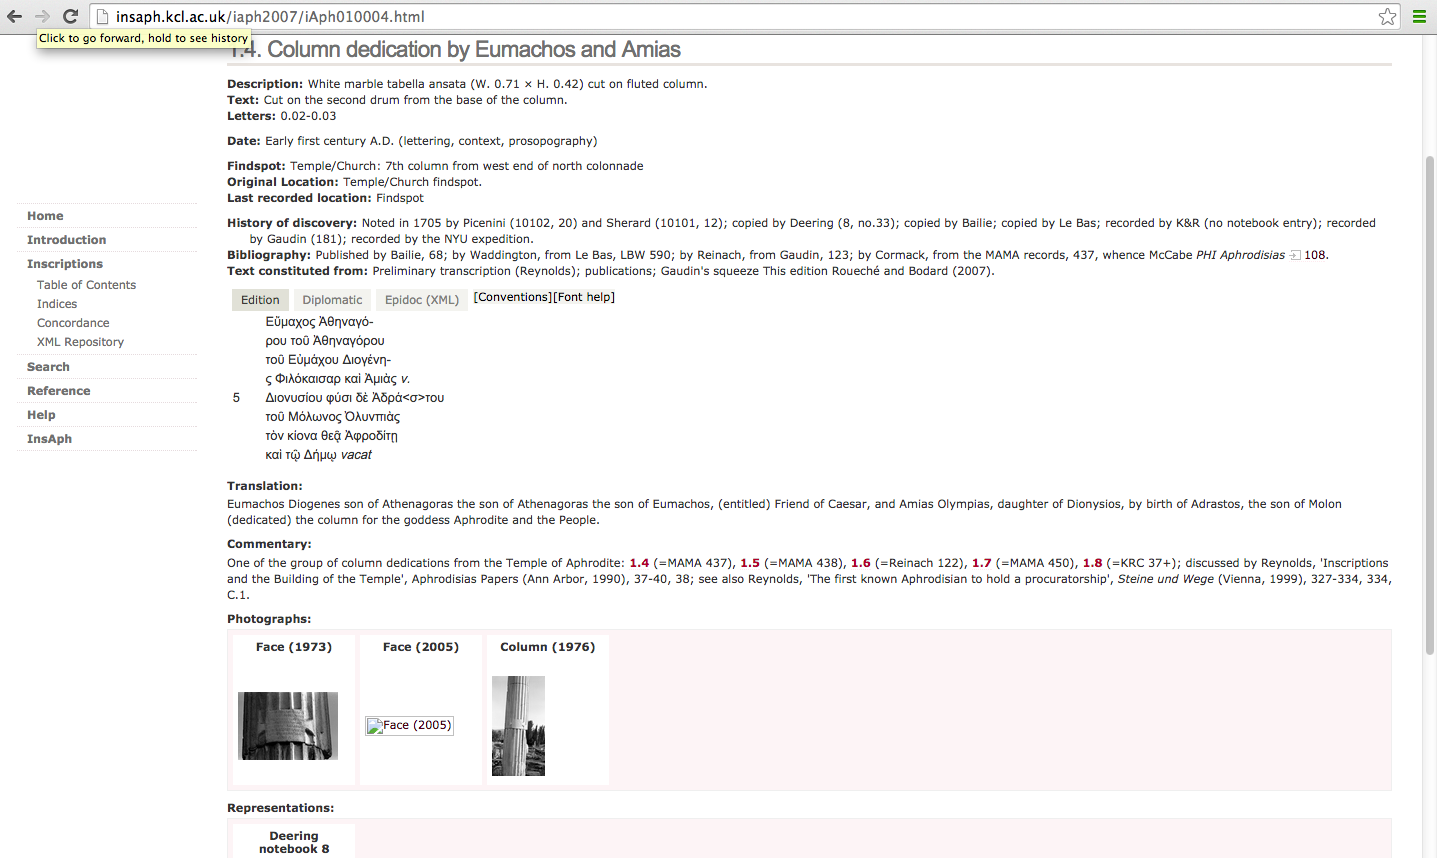
\includegraphics[width=0.7\columnwidth]{PaperproposalforEAGLEfinal-img001.png}
\caption{Screenshot of IAph 4 webpage}
\label{fig:1}
\end{figure}

\newpage
In addition to the format of the webpage, a number of images have been published along with a drawing from Deering’s
notebook from the early 19th century. \ These resources provide an opportunity not only to view the inscription but to
see how it has been studied over time. The dating of the inscription includes a list of the criteria upon which it was
based: lettering, context, prosopography, adding a degree of transparency to the dating process. While the lettering is
not subject to further description, the inclusion of weblinks to parallel texts allows the viewer to compare and
contrast different inscriptions, developing his/her understanding this element. 




The published texts of IAph 1.4 and MAMA 437 present one significant variation: the inclusion of space indicators within
the text. This practice allows the reader to see how the use of space relates with the text of the inscription,
particularly in the case of line 4, where challenges in the text (misspelling of Ammias and carrying over of a single
letter from the previous line), can be observed in the inclusion of a vacat at the end of the line.\footnote{ Vacats,
more sparingly employed in late Republican and Augustan inscriptions at Aphrodisias, usually serve a grammatical and/or
decorative function (e.g. giving distinction to a name or key elements/individuals in the text (cf. building
dedications at the Sebasteion IAph 9.1, 9.25, 9.112)). This vacat serves little grammatical function, and is likely to
be a result of the arrangement of the text/ omission in Ammias’ name. } The indentation on the last line also reveals
a left orientation of the line which is more common in Late Republican/Augustan texts at Aphrodisias (e.g. IAph 1.1,
1.7, 1.8 and 1.38), as opposed to the ``justified'' approach (indentations on both sides of the text to accentuate a name
or word), which is more common in later Imperial inscriptions at Aphrodisias. 
\newpage
\begin{quotation}
\noindent MAMA 437\\
\begin{otherlanguage*}{greek}
\noindent Εὔμαχος Ἀθηναγό-\\
ρου τοῦ Ἀθηναγόρου\\
τοῦ Εὐμάχου Διογένη-\\
ς φιλόκαισαρ καὶ Ἀμιὰς\\
Διονυσίου φύσι δὲ Ἀδρά\textlatin{<}σ\textlatin{>}του\\
τοῦ Μόλωνος Ὀλυνπιὰς\\
τὸν κίονα θεᾷ Ἀφροδίτῃ\\
καὶ τῷ δήμῳ.
\end{otherlanguage*}

\end{quotation}
\begin{quotation}
\noindent IAph 1.4.\\
\begin{otherlanguage*}{greek}
\noindent Εὔμαχος Ἀθηναγό-\\
ρου τοῦ Ἀθηναγόρου\\
τοῦ Εὐμάχου Διογένη-\\
ς Φιλόκαισαρ καὶ Ἀμιὰς\end{otherlanguage*} v.\\
\begin{otherlanguage*}{greek}Διονυσίου φύσι δὲ Ἀδρά<σ>του\\
τοῦ Μόλωνος Ὀλυνπιὰς\\
τὸν κίονα θεᾷ Ἀφροδίτῃ\\
καὶ τῷ Δήμῳ
\end{otherlanguage*} vacat
\end{quotation}

High quality images on the website facilitate connections between the published text and the inscription. In the image
of IAph 1.4 (Fig.~\ref{fig:2}), one can to observe how descriptive elements manifest themselves in an
inscription: how varying letter sizes (2-3 cm) represent a lack of uniformity and crowding as space becomes more
cramped, and how, after the beautifully spaced upper lines (lines 1-3) the carver struggled (line 4) to fit the letters
in, possibly noticing his spelling error only when there was extra space at the end of the line. \ 




\begin{figure}[!hbp]
\centering
 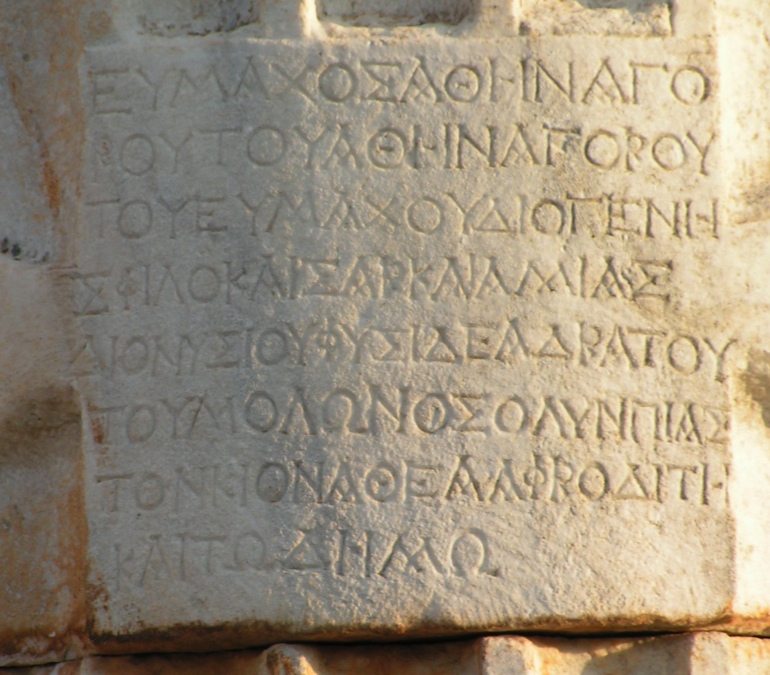
\includegraphics[width=\columnwidth]{PaperproposalforEAGLEfinal-img002.jpg}
\caption{Photograph of IAph 1.4}
\label{fig:2}
\end{figure}





Alongside spelling and the arrangement of the inscription, Letterforms are more readily observed. Overall, the lettering
is less uniform than later Imperial dedications, serifs are small and the strokes are both thick and deeply incised.
Letter height varies significantly as does the size of omicrons (though this can be seen in a poorly rendered text
throughout the Roman period). Angular forms such as alpha, lambda, and mu all intersect at the top meeting at sharper
angles than the more square versions of these letters that predominate in Imperial (post Augustan)
inscriptions.\footnote{ Compare with Hadrianic Lettering in the next section of the paper.} \ Letters also bear
stylistic elements of the time: epsilons have a connected middle bar (this is often disconnected in Imperial versions
of this letter), the rhos have small legs, making them appear more like their Latin counterpart, and the omicron has an
oval shape with serifs only at one end of the lower bars.\footnote{ ``Legged'' rhos are observed primarily in Augustan
and Julio-Claudian dedications and also on coins (cf. note 15). This style letterform is increasingly less common after
Flavian period at Aphrodisias. } Comparing these letterforms with parallel dedications at the temple (IAph 1.1, 1.2
(Zoilos’ dedications), 1.7 and 1.8) reveals many similarities. Letterforms alone are not diagnostic but when combined
with other elements, they can add to our understanding of a date. 







\subsection{Looks can be deceiving. When Inscriptions defy our expectations: IAph 1.5 and IAph 1.6.}
\noindent Based on the publication of these inscriptions in MAMA VIII, one could easily come to the conclusion that all the column
dedications at the Temple of Aphrodite looked quite similar. However, upon visiting the site of Aphrodisias in the
summer of 2004, I was (yet again) to be denied a simplistic interpretation of an inscription. Courtesy of the IAph2007
website, a broader audience can now bear witness to complex nature of these inscriptions. \ The first disparities
between the two inscriptions (IAph 1.4 and IAph 1.5) can be observed in a comparison of letter sizes. IAph 1.4 records
letters between 2-3 cm (with a variation of 1 cm), while IAph 1.5 varies only between 2.5- 2.75 cm (a variation of
.25cm). The reductions in variation of letter size are part of a general standardization in letterforms during the
Julio-Claudian period at Aphrodisias.\footnote{ These Julio-Claudian texts record little if any variation in the size
of letter forms. } While significant variations in letter size can be observed in poorly executed inscriptions
throughout Aphrodisias’ history, one may not expect such a significant variation between two ``copies''.\footnote{
\citep{graham2015} illustrates a further case study of ``copy'' inscriptions at Aphrodisias.} \ The published
text of IAph 1.5 also indicates indentations on both sides of the word demos in the bottom line. While double
indentations are not unknown in Augustan inscriptions at Aphrodisias, they are more common in later Imperial
inscriptions.\footnote{ Double indentations in an Augustan text are attested (IAph 12.301, dating to 23-25 BC), but the
practice is more common in Julio-Claudian dedications (Sebasteion: 9.34, 9.36, 9.37, 9.38, 9.39, The city wall 12.515
(Claudian)).} These discrepancies, which suggest that the two inscriptions may have been less similar in appearance,
illustrate the importance of reading the descriptive elements of an inscription carefully. 


\begin{quotation}
\noindent MAMA 438\\
\begin{otherlanguage*}{greek}
\noindent Εὔμαχος Ἀθηνα-\\
γόρου τοῦ Ἀθηναγό-\\
ρου τοῦ Εὐμάχου Δι-\\
ογένης φιλόκαισαρ\\
καὶ Ἀμμιὰς Διονυσί-\\
ου φύσι δὲ Ἀδράστου\\
τοῦ Μόλωνος Ὀλυν-\\
πιὰς τὸν κίονα θεᾷ\\
Ἀφροδίτῃ καὶ τῷ\\
δήμῳ.
\end{otherlanguage*}
\end{quotation}

\begin{quotation}
\noindent IAph 1.5.\\
\begin{otherlanguage*}{greek}
\noindent Εὔμαχος Ἀθηνα-\\
γόρου τοῦ Ἀθηναγό-\\
ρου τοῦ Εὐμάχου Δι-\\
ογένης Φιλόκαισαρ\\
 καὶ Ἀμμιὰς Διονυσί-\\
ου φύσι δὲ Ἀδράστου\\
τοῦ Μόλωνος Ὀλυν-\\
πιὰς τὸν κίονα θεᾷ\\
Ἀφροδίτῃ καὶ τῷ
\end{otherlanguage*} \\
vac. \begin{otherlanguage*}{greek}
Δήμῳ
\end{otherlanguage*} vac.
\end{quotation}



A high quality image (Fig.~\ref{fig:3}) illustrates further differences between the appearance of this inscription
and the comparative materials from the site (IAph 1.1, 1.2, 1.4, 1.7 and 1.8), revealing regular letterforms (e.g. omicrons are less oval and more precisely rendered
throughout) with a clear contrast between slender strokes and large deep triangulate serifs. There are no legged rhos,
the middle bars of the epsilons are separated from the stem, and the omegas are circular with two large bars that are
heavily serifed on both ends (e.g. compare the omega on the bottom line of IAph 1.4 with its counterpart of IAph.1.5).

\newpage

\begin{figure}[!hbp]
\centering
 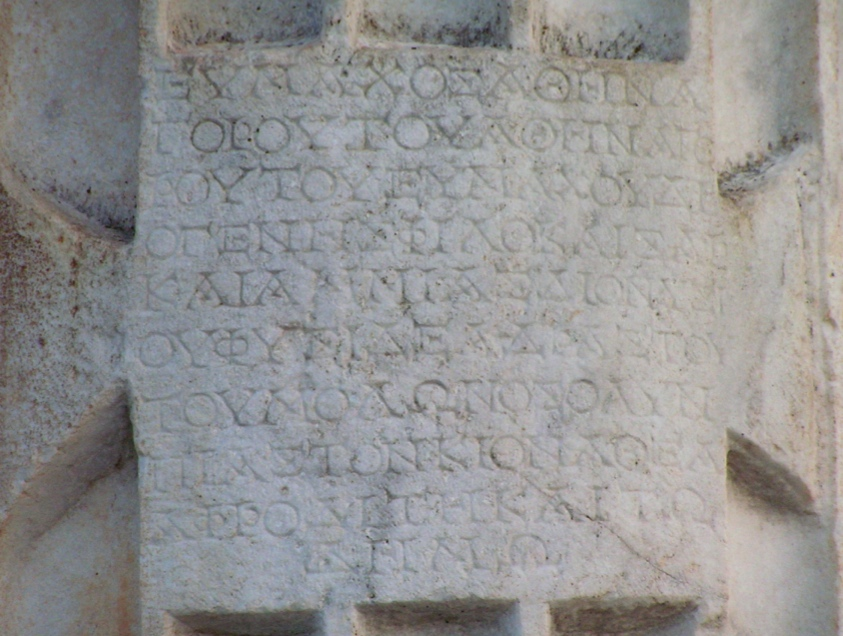
\includegraphics[width=\columnwidth]{PaperproposalforEAGLEfinal-img003.jpg}
\caption{Photograph of IAph 1.5}
\label{fig:3}
\end{figure}


These traits along with others (e.g. letter size and use of spacing noted above) are commonly attributed to late 1st
/2nd c. AD inscriptions at Aphrodisias, and are absent from comparative Augustan materials on the site (e.g. IAph 1.1,
1.2, 1.4, 1.7 and 1.8, including a Julio-Claudian dedication 1.102). Although one must be careful with stylistic
factors, especially when archaisms can be used, it is worth noting when a number of features that are attributed to a
later period, seem to suddenly emerge nearly a century early.\footnote{ Archaising and imitation of earlier lettering
is evident in at least one inscription (IAPH 13.116) \citet[155-166]{reynolds1982}). } Any one of these features, letter
variations, stylistic letterforms, use of serifs, indentations in the text, correction of errors in a previous text,
would not stand well alone, but taken together, a more compelling case can be made for the reassessment of this
inscription’s date. 




The website records the date of this inscription just like IAph 1.4: citing ``context, lettering and prosopography.'' For
those trying to gain an understanding of letterforms at Aphrodisias, this is somewhat confusing and it is not the only
example in which the lettering and organization of the inscription do not match date provided.\footnote{ Honours for
Zoilos (IAph 8.203) is dated by ``prosopography'' to the 1st c. BC but the letters are square Imperial forms and do not
match Zoilos’ other dedications (8.1, 1.1,1.2). Honours for P. and M. Vinicius (IAph 3.101) are dated as ``Augustan'' and
``Tiberian'' by ``lettering'' though prosopography is known (there is some controversy cf. Reynolds 1982,175). Stylistic
elements (arrangement, spacing and decoration), particularly in M. Vinicius’ base, reflect qualities of
Claudian-Flavian period inscriptions (which is not excluded by prosopographical dates). In both cases, conflicting
dating criteria are omitted. } The date of the text is not incorrect, insofar as it was originally inscribed at
this time and the prosopography as well as the formula of the text support this. However, one struggles to see how
the lettering and/or the arrangement of the text corroborate this date. An answer may be found in further examination
of the inscription’s context and prosopography. In addition to a number of earthquakes, new temenos of the temple was
added under the emperor Hadrian, a time during which Athenagoras’ descendants were alive and prospering in
Aphrodisias.\footnote{\citep[43]{smith1995}. For an analysis of the temenos plan, see \citet[66-74]{doruk1990}. For Athenagoras descendants, cf. note 17 and \citet[327-334]{reynolds1999}.} 




One benefit of the website is that it facilitates searches for parallel texts in this context and this period. A
Hadrianic building dedication from the temple, IAph 1.174 (Fig.~\ref{fig:4}) reveals similarly
rendered letterforms with little variation in size and a number of stylistic similarities: thin strokes with deep
triangulate serifs, the omicron with double serif bars, an epsilon with a separated crossbar. Similar observations can
be made on a number of Trajanic and Hadrianic texts at Aphrodisias (IAph 4.308, 5.9, 5.208 (Hadrianic Baths)). A theory
of later recarving would reconcile a number of disparities in this inscription. 







\begin{figure}[!hbp]
\centering
 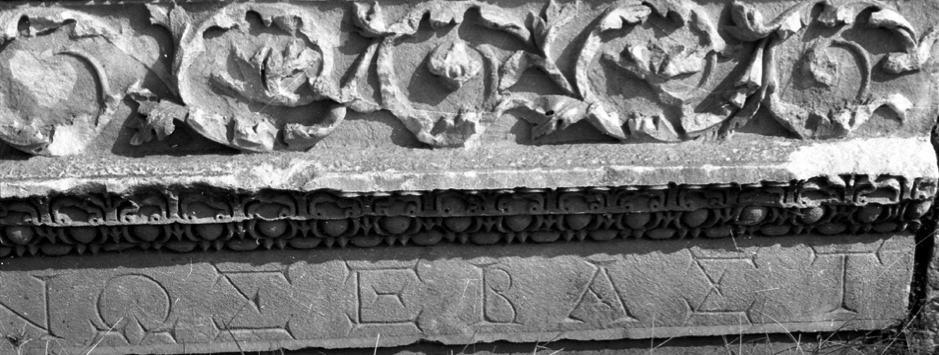
\includegraphics[width=\columnwidth]{PaperproposalforEAGLEfinal-img004.jpg}
\caption{Photograph of IAph 1.174}
\label{fig:4}
\end{figure}





This is not to say that IAph 1.5 was definitely a Hadrianic recarving, but to observe that, contrary to what is recorded
in the IAph2007 dating criteria of this inscription, the lettering and arrangement of text on the stone do not reflect
an inscription that is an obvious contemporary with the other column dedications at the temple. The context and
prosopography of the inscription do not rule out a later date and the text, which rectifies issues in both organization
and orthography of IAPh 1.4, reflects an inscription that may have responded to an earlier monument. 

The entry for IAph.1.6 represents a different response to a similar problem. It demonstrates that scholars are willing
to use letterforms to support a recarving when the case is sufficiently extreme. The text, only mentioned in MAMA VIII
as a ``copy'', presents a number of irregularities, repeating some errors, correcting others, and making quite a few new
ones. Whilst maintaining the first 3 lines of the arrangement in IAph 1.4, this inscription compounds the error on line
4 by reduplicating two letters in the name Diogenes. Line 5 repeats the misspelling of Ammias, corrects the misspelling
of Adrastos (line 6), but creates two new errors in line 7, missing out the nu on Molon and Olynpias, then repeating
the column phrase in lines 9- 10. 

\begin{quotation}
\noindent IAPh 1.6.\\
\begin{otherlanguage*}{greek}
\noindent Εὔμαχος Ἀθηναγό-\\
ρου τοῦ Ἀθηναγόρου\\
τοῦ Εὐμάχου Διογε-\\
\{γέ\}νης Φιλόκαισαρ καὶ\\
  Ἀμιὰς Διονυσίου φύσι\\
δὲ Ἀδράστου τοῦ Μό-\\
λω\textlatin{<}ν\textlatin{>}ος Ὀλυ\textlatin{<}ν\textlatin{>}πιὰς τὸν κί-\\
ονα θεᾷ Ἀφροδίτῃ \{τὸν\}\\
\{κίονα\} καὶ τῷ Δήμῳ
\end{otherlanguage*}
\end{quotation}


Reading this inscription is even more of challenge (Fig.~\ref{fig:5}), one can suffer vertigo as the
lines run up and down and the letters run into the margins. There is no use of spaces or decorations to clarify or
distinguish sections of the text and there are quite a few inadvertent errors to make it difficult, even to the trained
eye. Although the prosopography and context support an earlier date, the entry suggests that this ``inelegant'' text was
``recarved ?'' The entry does not, however, propose a date or explain why, in this instance, recarving is a viable
conclusion. While a methodology is evident in the IAph2007 dating format, it is not employed consistently or
transparently in this case. 


\begin{figure}[!hbp]
\centering
 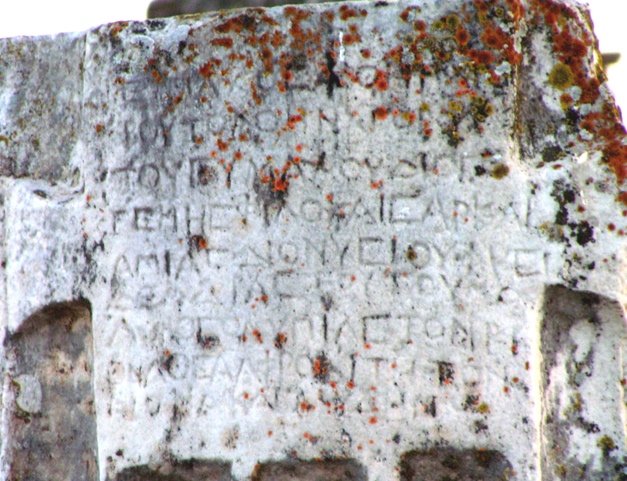
\includegraphics[width=\columnwidth]{PaperproposalforEAGLEfinal-img005.jpg}
  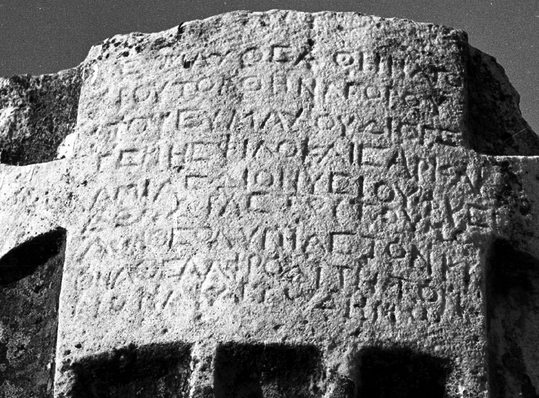
\includegraphics[width=\columnwidth]{PaperproposalforEAGLEfinal-img006.jpg}
\caption{Photograph of I.Aph 1.6}
\label{fig:5}
\end{figure}
 



The inclusion of numerous images proves crucial here, where moss now covers parts of the text that were legible in the
1970’s. The lunate omega on the bottom line (barely visibly in the recent photo) along with the lunate sigmas indicate
that the inscription is from the late Antique period at Aphrodisias, possibly after an earthquake in 359 BC (for
parallels see ALA 29 and 30), before the conversion of the temple into a Christian church (after 450 AD).\footnote{\citet[41-42]{smith1996}.} Acknowledging that the text was reinscribed centuries later affords further insight into both
the inscription and act of recarving as a process that often changed an inscription but did not necessarily improve it.





The three inscriptions betray fundamental differences, which reveal a rich and complicated tale of a column’s life at
Aphrodisias. While minor differences in the text do not change our translation of the words, a close analysis of the
resulting inscription informs our understanding of the arrangement of the text, the potential dating of the
inscription, as well as the relationship between text and monument. Recarving was not a highly unusual phenomenon in
the ancient world but by minimizing the conflicting elements of these inscriptions, one potentially overlooks this
aspect of an inscription.\footnote{\citet[135-177]{thomas1990}.} 




\subsection{Conclusions on the case study}
\noindent This survey of column dedications has demonstrated how a series of inscriptions, which were represented as a series of
similar texts in MAMA VIII can be seen in a fundamentally different way in IAPh 2007. The digital publication has a
number of advantages: it applies a more rigorous approach to the text in XML thus illustrating the arrangement of the
inscription more clearly, the date is given some transparency through a list of applied criteria, and the descriptors, such
as the lettering size of the inscriptions, provide more information. The images of the inscription in drawings and its
context provide an invaluable resource that allow the reader to better understand the relationship between text,
inscription and context, including references and better accessibility to parallel inscriptions. In terms experiencing
an inscription in a digital world, this is probably as close as a person can come to assessing the face value of an
inscription. It is a tremendous step forward in addressing the longstanding limitations inherent in the publication
of epigraphic evidence, though some challenges remain. The final section will consider how we might further use this
information, in terms of adding clarity and transparency to the dating process, as well as in our approach to these
materials.




\section{Palaeography in a Digital World: Monumental Problems \& Solutions}

\subsection{Digital Epigraphy. New Method: New Methodology?}
\noindent For students and academics alike, dating by letter forms is an almost ``mystic'' practice: something upon which experts
often comment but more rarely explain or demonstrate in practice. Recent epigraphic handbooks keep the term
palaeography at arms length, using it interchangeably with discussions of letterforms.\footnote{In the index \citep[880]{bruun2015} ``palaeography'' is cross-referenced with ``Letter forms'' and though used by O.
Salomies (chapter 9), the word is not defined in the preceding chapters \citep[155]{bruun2015}.
Letterforms are described generally with charts of figure numbers rather than images to directly illustrate changing
styles (\citep[123-4]{bruun2015}). Cooley’s manual offers a more detailed assessment of lettering with case studies to
illustrate the limitations of using lettering \citep[423-33]{cooley2012}} The caution of these scholars is justified and
understandable: conclusions based on a single element of an inscription are precarious and, perhaps more importantly,
they represent a mode of scholarship that views inscriptions in a fundamentally different way than they were viewed in
antiquity. Writing, both ancient and modern, is a product of a number of factors, all of which functioned together in
the image of writing (margins, lettering, indentations punctuation).\footnote{\citet[25-27]{woolf1996}, \citet[3-5]{bodel2001},
\citet[433-437]{cooley2012}; \citet[1-10]{panciera2012}.} As few would look at a document today and say ``that’s a fine Helvetica
10 point!,'' we should be cautious in an assessment of palaeography that excludes the visual elements which were
inextricably linked an inscription’s appearance (e.g. alignment, margins, spacing, punctuation). Modern definitions and
studies of manuscripts suggest a broader scope of inquiry, which includes handwriting together with decorations and
spatial organization as well as subsequent comments in the margins.\footnote{\citet[21-37]{buonocore2015}. } These
practices suggest a discipline with an interest not only in the evolution of lettering but in the appearance and
development of a culture of writing. 



\newpage
While traditional text-based modes of publication such as MAMA VIII have, at times, constrained the study of hands to an
analysis of lettering, digital corpora offer new opportunities to view, analyse and incorporate broader scope of visual
elements in the interpretation of an inscription. This is not to say that the traditional methods or charts of
letterforms development should be abandoned, merely that the methodology could be expanded, as it has been in this case
study, to include aspects of textual organization (spacing, use of decoration and punctuation, letter size). The
question arises: how do we achieve this through the website materials? 



\subsection{Employing change: How we might improve presentation of materials on the website.}
\noindent One difficulty of the current site, observed in the assessment of IAph 1.5 is that despite the clear criteria for
dating, the terms do not reflect a consistent methodology in dating, or the contradictions in the process. This is
dangerous for those who simply accept the dates provided, and confusing for those who try to apply or develop a sense
of letterform development. When a recarving is suggested IAph 1.6, there is little to explain how we know it was
recarved (letterforms) or when the recarving took place (use of parallel texts), though both resources are available on
the website. The wealth of visual, textual and contextual information in IAph 2007, offers an opportunity, not only
clarify, but to add greater transparency to the process of dating and how lettering is used in an inscription. This
could be achieved by adding a few pages to explain and illustrate elements dating criteria (each with a significant
Caveat Lector on the use of these elements). Firstly, one could add a page outlining the dating criteria, providing a
brief description of each (e.g. context, lettering and prosopography) together with a sample case study (or two) of how
these factors are applied in an inscription. 




\ Further improvements, could be made with additional pages on lettering and context. \ While lettering is undoubtedly
employed in dating inscriptions at Aphrodisias, one must also consider how this dating is represented in the published
materials. Epigraphers, who have described monumental lettering as `Augustan', `distinctively Julio-Claudian' or
`Domitianic' have already acknowledged that such distinctions exist at Aphrodisias, but the classifications remain
undefined.\footnote{ Studies of inscriptions describe lettering as ``distinctively Julio-Claudian'' \citep[nos. 2\&3) 317-318]{reynolds1982}, ``Triumviral or Augustan'' \citep[docs. 35-37, 159-163]{reynolds1982}, and ‘Domitianic’ \ (Chaniotis 2004, no.
14), suggest that such distinctions are evident at Aphrodisias.} While such definitions are often problematic, so is
a situation in which a broader audience accepts and uses a series of dates, without understanding how certain criteria
have been used in formulating a date. Undertaking a detailed palaeography for a site is a massive endeavor, and one
that can prove contentious on a number of levels. However, a page about lettering (together with aforementioned element
of textual organization) could be added with brief descriptions of trends (periods of ca. 60-70 years) and references
to a few inscriptions as illustrations. This could be supported by a single case study, such as this one, to show how
these elements are used as well as how they can be problematic.



Finally, while inscriptions are given a good deal of context in IAph 2007, the epigraphic information remains
separated from the archaeological studies. Both of these are factors in the dating process and, as we observed in IAph
1.5 and 1.6 can often facilitate the study of an inscription, both in reconciling discrepancies and searching for
parallel inscriptions. With inscriptions grouped by context and an excavation history that is referenced (but not
explained) it might be helpful to have a brief building history for each context. In the case of Aphrodisias, these
materials and further bibliographies are available on NYU excavation websites and could be easily connected with
weblinks.\footnote{ NYU website. \url{http://www.nyu.edu/projects/aphrodisias/home.ti.htm}. Recent excavation reports are
reference here as well: \url{http://www.nyu.edu/gsas/dept/fineart/academics/aphrodisias/aphrodisias.htm}.}




The benefits and the challenges observed in the IAph 2007 digital publication are applicable to a number of digital
resources. As we attempt to bring corpora of unprecedented size to a digital realm, we must consider not only how we
represent this information but how we engage a wider readership in epigraphic materials. It would not take a great deal
of work to augment the scope of IAph 2007 from an academic resource into one that also achieves a didactic aim of
illustrating how we use different elements of an inscription (including letter forms) to suggest a date for an inscription. The point is not necessarily to establish a firm date, but to provide greater transparency to process by which we formulate dates. We have the potential now, to present inscriptions at
face value, not only as texts but as contradictory objects whose stories, whether conveyed on stone or a computer app,
are subject to the same conventions, complexities and imperfections as the humans who created them. 

\nocite{roueche2004} 
\nocite{buraselis2000}
\nocite{bruun2015}
\nocite{calabi1991}
\nocite{chaniotis2004}
\nocite{calder1962}
\nocite{panciera1995}

\bibliographystyle{sapauth-eng}
\bibliography{../../EAGLE}

\end{document}
